\part{古典经济思想及其批判}

通常所说的经济学古典时期,涵盖了一百多年的经济思想,其方向与主要贡献者几乎为英国
人所垄断。

从1776年到1820年几乎是斯密时代,从大约1820年到19世纪50年代是李嘉图时代,从19世纪
50年代到19世纪90年代是约翰·斯图亚特·穆勒时代。

另外两位先行思想家是马尔萨斯与马克思,尽管他们在某些方面来看属于古典学派,但是与
作为古典经济学的拥护者相比,他们作为古典经济学批评家的意义更大。马尔萨斯的人口理
论符合古典理论,但是马尔萨斯在他对经济体某些宏观方面的分析中,以及在他对地主阶层
的作用与重要性的捍卫中,却引人注目地背离了正统的古典传统。但是,我们将单独考察马
尔萨斯与李嘉图之间关于经济体自动实现资源充分利用的著名论战。卡尔·马克思从古典经
济学中汲取了一些因素,加入了不同的看法和一些新的分析概念,得出了与古典理论及政策
直接相对立的结论。

\subsection{古典政治经济学}

与重商主义思想最大的不同是,他们对经济力量自然运作所产生的结果持赞同态度。在古典
经济学家眼里,经济体制通常是和谐的,这与重商主义者与经院哲学的信仰尖锐对立,重商
主义者与经院哲学均认为市场的特征在于不和谐,需要进行限制和干预。

法国重农主义者最早引人注目地提出了下面的观点,即针对相对稀缺性产生的冲突,市场自
动地提供和谐的解决办法……政府应当对经济体采用自由放任的政策……

古典学派确信借助自由这一手段,经济体能够最有效率地运行。他们断言,个人与厂商应当
不受政府干预地自由交易。除此之外,古典学派认识到,政治自由与经济自由是不可分割地
绑在一起的,亮着彼此影响。

但他们也非常了解社会冲突,尤其是地主与那些提倡经济增长与变革,并从中获益的人之间
的冲突。正像斯密与李嘉图两人所理解的那样,资本主义的长期趋势导致了这些不和谐的后
果。

经济体制中和谐概念相关的两条显著的发展路径。一方面是,主流正统经济思想尽管一直不
断地接受和谐运行的经济体制这一基本前提,却正通过越来越多地鼓吹经济问题的政治反应
而非经济反应,缓慢而稳定地弱化这一前提。另一方面,一些非主流经济学家否认古典经济
学所认同的和谐性,并发现了体制中的一些基本冲突,这些冲突需要对制度结构进行主要变
革才能加以解决。马克思主义思想是下面这种经济思想最重要的例子,即认为经济体制充满
了矛盾冲突,通过市场力量无法予以解决。

古典经济学派的第二个特征是它对经济增长的关注。……宏观……所以古典经济学家致力于
发掘决定经济增长率的力量、文化、政治、社会、历史因素。这方面凯恩斯主义者的主要关
注点是决定经济活动水平的力量。他们考虑某一时点上一个经济体是否在低于资源充分利用
的水平上运用。古典经济学派对这一问题并不感兴趣,因为他们已经假设经济体倾向于在资
源充分利用的水平上运行。当现代宏观经济学背离凯恩斯主义宏观经济学时,又回到了这些
相同的问题与假设上来,所以,现代宏观经济学家有时也被称为“新古典经济学家”。

古典经济学家对增长的关注使得他们去研究市场,研究作为资源配置者的价格体制。……古
典学派延续了重商主义者的传统,因为两者都聚焦于我们今天所谓的“宏观经济学”。

相比古典经济学,新古典经济学在比较静态的框架中研究市场,目的是使下面的这些问题更
加清楚,即什么力量决定了相对价格,生产了什么种类与数量的消费者产品,利用了什么种
类与规模的经济计划,收入的个人分配与功能分配是如何决定的。直到19世纪70年代,初生
的新古典经济理论才将经济学家的注意力从增长上引开,几乎专门研究有关在供选择的用途
之间分配稀缺资源的微观经济问题。

斯密经济学的最后一个统一特征代表了与重商主义思想的显著背离。尽管重商主义者的理论
结构是不牢固的,但是他们相信自己有能力了解经济体的运行。一旦他们认为自己获得了这
方面的知识,就会认为对他们所洞察的经济体运行中的任何缺陷进行修补是合适的。这种修
补要么通过变更制度结构,要么通过允许政府干预来实现。……重商主义者的角色认知与亚
当·斯密的怀疑论完全相对,斯密向胆敢以其判断来替代市场判断的政治家贤人提出了质疑。

\subsection{马克思的政治经济学}

卡尔·马克思是古典经济学最重要的批评家,也是打造古典(classical)一词的人。马克思
是经济思想史的学生……影响马克思的最重要的经济学家是李嘉图。尽管古典经济学派发现
经济体是基本和谐的,并因此提倡自由放任的政府政策,但他们同时也发现了很多冲突。其
中之一就是地主与资本家之间的冲突。马克思指向资本家与劳动者之间的经济冲突。他改造
了古典学派的劳动价值理论以支持他的观点,即劳动者受到资本家的剥削。

古典经济理论与新古典理论不同,其分析的事物与结构是动态的。亚当·斯密集中研究经济
增长,大卫·李嘉图对资本主义中发生的收入分配的长期变化感兴趣。马克思的经济分析只
是其兴趣点的一部分,他的兴趣点是引起历史变革的力量。然而,古典学派所研究的一些相
同的动态问题,也引起了马克思的兴趣,例如,随着时间的变化,收入分配发生怎样的变化,
利润率将采取怎样的进程,大众福利水平的前景如何。

李嘉图和马克思都对劳动价值论感兴趣,但并不是因为它解释了某一时点上什么力量决定了
相对价格,也不是因为它把在可替代的用途之间有效分配稀缺资源的问题说得更清楚。马克
思想表明,剥削是如何根植于劳动者不拥有生产手段的体制中的;李嘉图则运用劳动价值论
来解释随着时间的变化收入分配的变化。

马克思对古典经济学的另一借鉴:对古典学派来说,主要的参与者是资本家、地主、劳动者。
在某种意义上,古典理论是对经济运行和对这些阶级的未来的一种分析。古典学派与马克思
都将社会中的动态因素视为资本家阶级活动的结果。

古典学派与马克思之间的差异比他们的相似之处更加显著,他们之间最重要的分歧是相互抵
触的意识形态上的观点。古典学派发现,资本家的利润动机导致经济体中资本的有效配置,
并导致储蓄,这将促进经济的增长和财富的增加。马克思则将资本家的活动看做是最终有害
于无产阶级和社会的。

\chapter{亚当·斯密}

\section{亚当·斯密的博学多才}

经济学家、大学教师。私密讲授一系列课程,其中包括我们现在所称的社会学与人类学,他
主要对道德哲学感兴趣。他注意到经济自由与政治自由之间的重要关系,私人财产权利与公
正状态之间的重要关系,以及由利己主义所推动的个体与由关注其行为对他人产生的后果所
推动的个体之间的重要关系。

曼德维尔的讽刺风格令其对重商主义立场的表述广为流行。曼德维尔与斯密都是从人类利己
本性这一相同的假设出发,但却得出了相反的结论。曼德维尔主张,个人对私利的追求,会
产生很多不良的社会和经济后果,因此他为政府干预经济构建了一个实例。

斯密所处的时代,已有的不同研究领域之间不存在清晰的界定:哲学、自然科学、社会科学、
道德都被当做真理统一体的不同方面来对待,而不是当做单独的学科。此外,从事研究的知
识精英受到了严格意义上的教育,他们被要求掌握最宽广的人类知识。

这种多学科方法的一个后果是,那些像亚当·斯密一样,主要探求我们现在称为社会科学与
道德知识的人认为,牛顿在物理学中所建立的科学严密性,在他们主要努力的领域中也能够
达到。显然,斯密及其同时代的人,能容易地把今天被称做实证性的问题与规范性的问题相
混合。

斯密对经济学范围的认识,继承了英国重商主义者的观点。他对解释国民财富的性质与原因
感兴趣。现代经济学家将斯密描述为对决定经济增长力量感兴趣的宏观理论家。然而,斯密
所考察的力量比现代经济学家所研究的力量要宽泛,他用政治的、社会的、历史的材料来填
充其经济模型。他注意到了相对价格的决定——今天包含在微观经济理论中——但是,它的主要
兴趣在经济发展与推动经济增长的政策上。

因为斯密断定经济体总是充分使用其生产资源的,所以,他没有触及宏观经济学中的一个重
要问题:当经济体的生产能力既定时,什么力量决定收入与就业水平?

斯密将演绎理论与历史描述相结合的方法论也值得注意。他的理论模型缺少优雅与严密,但
是,他对经济体中的相互关系和经济体运转的描述,以及他将历史实例组合进分析中的能力,
是无可比拟的。

\subsection{新教与资本主义:是否是一种因果联系}

R.H·托尼《宗教与资本主义的兴起》,马克思·韦伯《新教伦理与资本主义精神》认为宗教
改革与新教伦理观的兴起,极大地促进了产业革命与资本主义的出现。我们已经了解,天主
教教义的根源在亚里士多德,它与新产业秩序的成长相敌对。但是,约翰·加尔文及其追随
者的教义,确实与经济活动兼容的。韦伯--托尼的论题是宗教直接有助于资本主义体系的兴
起。韦伯与托尼受到很多经济学家的批评,然而,他们两人都是细致小心的学者。他们承认,
在宗教观点、经济行为以及经济制度之间确定因果关系的次序是极为困难的。例如,他们认
识到,因果关系也会涵盖在从经济制度到宗教观点中,产业革命与资本主义的发展可能同等
程度地说明了新教伦理观的发展与认同。

经院哲学教条主张,表现为个人财富的经济活动的成功,是罪孽行为的强烈指征——索要过高
的价格,以高利率放款,过分注重收益却少关注灵魂救赎。根据经院哲学伦理观,经济活动
的成功显示了永恒拯救的语言。经院哲学还认为,努力工作有益于灵魂,炫耀性消费应当予
以避免。强调劳动与节俭美德的宗教观点,被认为是促进现代经济社会出现的主要因素。

\section{斯密的市场分析与政策结论}

有两种可行的方法来分析亚当·斯密的著作。一种方法是考察整体的理论结构与政策含义,
这些政策含义或者内在于理论体系中,或者由斯密明确地予以表述。另一种是详细地考察理
论结构,来评价理论内在的一致性抑或一致性的缺失(专注于理论技巧方面)。本书专注于
第一种方法,全面地考察斯密的理论结构,同时考察从更详细的经济分析中产生的政策结论。

斯密作为一位经济学家的强大实力在于,他洞察了:(1)经济体组成部分的相互依赖;(2)
用来推动一国财富的政策。

\subsection{前后关联的经济政策}

斯密提倡自由放任,并不是因为他认为市场是完美的,而是因为联系到他所处时代英国的历
史与制度结构,市场通常会比政府干预产生更好的结果。

斯密是经济学艺术大师。前后关联的经济政策(contextual economic policy),就是另一
种表达经济学艺术观点的方式。后来的经济思想家在方法上有所改变。李嘉图对自由放任的
倡导是前后不关联的,这与其抽象的无历史记载的方式相一致。穆勒与马歇尔回归到斯密的
传统上来,在所做的分析与政策结论中,他们明智地设法将理论、历史与当时的制度相结合。

现代经济学正在偏离抽象的理论化,很多现代经济学家与政治学家正在考察政府与政府政策
如何才能实际发挥作用。这些现代公共选择理论家们劳动的一个无意识结果,可能就是重新
引起人们对前后关联的经济政策——经济艺术的兴趣。

\subsection{自然秩序、和谐与自由放任}

受到物理学发展的影响,重商主义者和斯密认为,依靠严格的分析是有可能发现经济体的规
则的,他们都就人类本性作出相同的假定:人类是有理性的,是有私心的,很大程度上受经
济利己主义的驱使。

斯密体系与大多数重商主义者体系的一个区别在于他的假设,即竞争性市场在极大程度上是
存在的,在这些市场内部,生产要素自由流动,从而提升了它们的经济优势。第二个区别是
下面的假设,即经济体的自然运转过程,能够比人类做出的任何安排更有效地解决冲突。

\begin{quotation}
  他受着一只看不见的手的引导,去尽力达到一个并非他本意(人的自利)想要达到的目的。
  并非其本意对社会来说不一定是坏事。他追求自己的利益,往往能使他比在真正出于本意
  的情况下更有效地促进社会的利益。我从未听说那些假装为公共利益而从事贸易的人会做
  什么善事。的确,这种虚伪在商人中间并不常见,所以,基本不需要费什么口舌来劝阻商
  人的这种虚伪。
\end{quotation}

斯密得出其主要政策结论的推论法非常简单。人类是理性的,是有私心的,受利己主义的驱
使。如果放任不管,每个个体将追求他或她自身的私利,在促进私利的同时也促进了社会利
益。政府不应当干预这一进程,而应当遵循自由放任的政策……资本家是根据最终产品来看
待市场的,为了增加收入而生产人们所期望的商品。资本家之间的竞争,将使这些产品在某
一生产成本下生产出来,这一生产成本将返还生产者正好足够支付不同生产要素机会成本的
一个数量……消费者通过他们在市场上的货币选票来引导经济体;消费者欲望的改变在价格
的上升和下降——因而在利润的上升和下降中得到体现。斯密断定,在没有计划和政府指导的
情况下,市场如何导致消费着欲望在最低可能的社会成本上得到满足,这将是一个其妙的过
程。按照现代经济学的术语,斯密断定,在没有政府干预的竞争性市场上会出现资源的最佳
配置。

\subsection{竞争性市场的运作}

斯密能够比以前的经济学家更准确地详细说明,源于竞争的价格在长期中为什么等于生产成
本这一道理。在他对价格形成与资源配置的分析中,他将短期价格称为“市场价格”,将长
期价格称作“自然价格”。他主要关注长期自然价格的形成。……因而产生的自然价格将使
资源得到最佳配置,原因在于消费者以最低的可能成本获得了他们想要的产品,同时,最大
的增长率得以保证。

确立了竞争性市场的优越性之后,斯密便毫无困难地构建起他反对垄断与政府干预的论
据。……他意识到垄断者将会通过限制产量来索要较高价格。值得注意的是,斯密提倡的自
由放任是以竞争性市场的存在为假定性条件和准则的。

私密反对政府干预经济的主张具有政治的、哲学的、经济的基础。他认为,一般而言,任何
政府干预都是不合意的,原因在于它侵害了个人正常的权利和自由。……斯密认为,尽管重
商主义者关于政府干预的很多主张都声称促进了社会利益,但其实是增进了个人私利。对国
内与国外商业的管制,不是有利于国家,而是有利于商人。……鉴于政府的运作方式,它们
将不可避免地有害于而不是有益于社会利益。从这个意义上讲,现代公共选择理论的根源,
可以追溯到亚当·斯密关于商人如何利用政府使自己富足的认识上。

然而,斯密对自由放任的拥护是有所限定的,因为他引用了几个领域,并认为在他所处时代
历史的、政治的、制度的背景下,在这些领域实行政府干预是必要的。例如,保护幼稚产业
的关税;政府应当提供国家防卫,修建并维护道路和学校,维护公正以及进行人口登记。更
重要的是,斯密提倡政府提供具有极大社会有益但私人市场因为没有充足利润而不去提供的
产品,以此来限定他对自由放任的主张。例如,教育。如果听任市场调节,那么市场所提供
的教育将少于社会所需要的(现代福利经济学的大量内容涉及外部性、第三方或溢出效应,
以及如果获得最大社会福利该如何考虑这些问题)。

在倡导自由放任政策的过程中,斯密非常谨慎。只有当竞争性力量存在并将私利引向社会利
益时,看不见的手才用来结合公共利益与私人利益。

\subsection{资本与资本家}

他指出,一国的现有财富取决于资本积累,原因在于资本积累决定了劳动分工和参加生产性
劳动的人口比例。其次,斯密断定资本积累也会导致经济发展。再次,与资本积累相结合的
个人私利导致资本在各产业之间的最佳配置。

资本家在经济体运行中扮演着主要角色。他对财富与利润的追逐,引导着经济体实现资源的
有效配置与经济增长。在一个私有财产经济体中,资本的来源是个人储蓄。斯密认为,劳动
并不能够积累资本,原因在于工资水平仅仅能够满足直接的消费欲望。他观察到,部分地主
阶级拥有足够的收入来积累资本,但是,他们却将这些收入花在非生产性劳动上,以满足他
们奢侈生活的无限欲望。……一部分正在兴起的产业阶级是对社会有益的人,他们为了利润
而奋斗,努力积累资本,通过储蓄和投资来增加他们的财富。因此,有利于资本家的收入不
平等分配,具有巨大的社会重要性。没有收入的不平等分配,就不可能有经济增长,因为全
部的年产出将被消费掉。

\subsection{斯密对政策的影响}

它的主要政策结论是政府应当接受自由放任的政策。这一结论对工业化国家的经济政策影响
巨大。它已经成为社会的经济意识形态……可以说,没有哪一个观点,没有哪一个经济学家,
对经济与社会的发展产生过更重要的影响。

\section{国民财富的性质与原因}

在《国富论》第一句中,斯密解释了国民财富的性质这一概念。这样他就将自己的观点与重商
主义者和重农主义者的观点区别开来。

\begin{quotation}
对每一个国家来说,供应全国人民每年消费的生活必需品与便利品的根本来源,是全体国民
每年的劳动;那些被消费掉的必需品与便利品,如果不是由该劳动直接生产出来的,便是用
该劳动的产出物向国外购买的。
\end{quotation}

在《国富论》全书的很多地方,斯密严厉指责重商主义者关注金银的积累,以及将金银等同
于一国的财富。……财富是产品与服务的年流量,而不是贵金属的累积储备量。他也揭示了
出口和进口之间的联系,认识到出口的基本作用是支付进口。此外,在他的开篇语中,他暗
示说经济活动的最终目的是消费,在《国富论》后面的章节中,他就这一立场予以了给全面
的阐释。这就进一步将斯密的经济学与重商主义的经济学加以区分,后者将生产视为其本身
的目的。最后,在强调劳动是一个国家财富的源泉时,斯密又与重农主义者不同,后者强调
的是土地。

\begin{quotation}
  消费是所有生产的唯一目的与意义;生产者的利益应该受照顾,但不该超过也许是促进消
  费者利益所必要的程度。……但在重商主义里,为了生产者的利益,消费者的利益几乎不
  断的被牺牲;它似乎认为,所有勤劳与商业活动的最终目的与意义,在于生产,而不在于
  消费。(《国富论》第四卷第八章末尾)
\end{quotation}

斯密继而建议,国家的财富应当按照人均指标来衡量。其实,斯密的这一看法一直被继承到
现在。

\begin{quotation}
消费是所有生产的唯一目的与意义;生产者的利益是应该受照顾,但不该超过也许是促进消
费者利益所必要的程度。此一箴言是如此纯然不证自明,只有想法荒谬的人,才会想要加以
证明。但在重商主义里,为了生产者的利益,消费者的利益几乎不断的被牺牲;他似乎认为,
所有勤劳与商业活动的最终目的与意义,在于生产,而不在于消费。

就限制所有可能和我们自己的产物或制造品一起竞争的国外商品进口而言,国内消费者的利
益显然是生产者利益的牺牲品。完全是为了后者的利益,前者才被迫承受这种独占几乎总是
会带来的价格上升的压迫。(谢宗华、李华夏所译《国富论》527页)
\end{quotation}

\subsection{国民财富的原因}

斯密主张,一个国家的财富即我们今天所称的一个国家的收入,取决于:(1)劳动生产力;
(2)有效使用或者生产性使用的劳动者的比例。因为他假设经济体将自动实现资源的充分
利用,所以他只考察那些决定一国产品与服务生产能力的因素。

\begin{description}
\item [劳动生产力] 在《国富论》第一篇中,斯密阐述了劳动生产力取决于劳动分工,强
  调这一原理。尽管斯密认可专业化与劳动分工的经济利益,但他也察觉到一些严重的社会
  成本。劳动分工的一个社会缺点是工人被赋予重复性的任务,这些任务很快就变得单调乏
  味。人们成了依赖于生产过程的机器……而失掉人性。但是,斯密毫不怀疑最终通过劳动
  分工增加了人类福利。

  劳动分工依次取决于斯密所谓的市场范围(extent of the market)与资本的积累。市场
  越大,可销售的数量越多,劳动分工的机会就越多。……劳动分工受到资本积累的限制,
  原因在于生产过程是耗时的:随着劳动分工的增加,劳动者不在为其自身的消费生产产品,
  在耗时的生产过程中,必须保持一定的消费品储备来维持劳动者。这一数量的产品来自于
  储蓄,即斯密所谓的资本。资本家的一个主要功能是为缩短生产开始与最终产品销售之间
  的时间间隔而提供手段。


\item[生产性与非生产性劳动] 根据斯密的观点,资本积累也决定了生产性劳动者与非生产
  性劳动者之间的比率。斯密对是否生产性劳动的尝试另其困惑,也反映了他所做出的规范
  或价值判断。然而,它也表明斯密意识到经济增长的问题。他主张生产可销售商品所使用
  的劳动是生产性劳动,而生产服务所使用的劳动则是非生产性劳动。资本家有益于经济增
  长与发展;而地主在仆人和其他无形产品上的花费、司法与军事人员等则是浪费。“资本
  因过度借鉴而增加,因挥霍浪费和不正当行为而减少。”

  斯密强调,通过下列分配方式,可以获得最高的经济增长率,即将大量收入分配给储蓄和
  投资的资本家,而将少量收入分配给地主,因为他们将钱花在仆人身上,并且“没有留下
  任何东西作为消费的回报。”此外,因为经济增长受到政府非生产性劳动支出的约束,所
  以较小政府就可以给政府征收较低的税,以便他们能够积累更多的资本。
\end{description}

\subsection{对国民财富原因的总结}

\begin{figure}[ht]
  \centering
  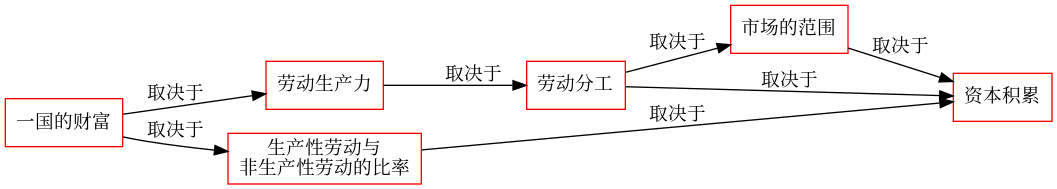
\includegraphics{simi.png}
  \caption{\label{fig:simi}一国财富的决定因素 }
\end{figure}

增加劳动力,通过机器工具或者劳动分工等提高已雇佣的劳动者的生产力,几乎都需要追加
资本。

对亚当·斯密来说,资本积累毫无疑问要求一个自由市场与私人制度框架。……在私人财产
体制中,对高资本积累率的进一步要求就是不平等的收入分配。

\section{国际贸易}

斯密主张非规制的对外贸易,理由是如果两国各自用生产成本较低的产品去交换生产成本较
高的产品,这种交换对双方来说都是有利的。用经济学的语言来说,这就是著名的对外贸易
的绝对成本学说。而且,这一学说不局限于国际贸易,它也适用于一个国家的内部贸易。

用现代经济学语言来说,随着劳动变得越来越专业化,存在收益递增(成本递减)的情形。
斯密认识到,如果两个个体出生时拥有相等的天赋并保持这一天赋不变,如果他们实行分工
并交换其产品,那么,他们中的任何一个人都不具有优势。然而,如果两个个体通过劳动专
业化变得更加熟练,那么两人所生产产品的成本都减少了,两人都从专业化与贸易中获益。
从斯密的这一见解中,产生了如下对自由贸易的发展至为关键的共识,随着时间的变化,任
何国家都能够通过专业化与劳动分工自动得获得生产某些产品的绝对成本优势,并且所有国
家都能够从此产生的国际贸易中获益。斯密认为,自由放任的政策将不断导致所有国家更高
的福利水平。

斯密在其广泛的社会科学与历史框架中,就经济分析做出的较少抽象而更多制度性的见解,
以及所使用的方法,直到今天还吸引着越来越多的注意力。政治经济学这一术语从经济学行
话中已经消失一百年了,但是,很多经济学家现在正迫切要求回归到更加斯密化的经济学范
围中,就像属于所暗示的那样。公共选择理论与新制度经济学两者的根源都能追溯到亚当·
斯密。

\section{价值理论}

价格或价格

(1)是什么决定了一件产品的价格?用现代经济学的语言来说,是什么决定了相对价格?(2)
是什么决定了价格总水平?(3)什么是福利的最佳度量标准?第一和第三个问题是现代微观
经济学的部分内容;尽管第二个问题难以用通常简单的“宏观--微观二分法”来判断,但是
一般情况下它都被包含在宏观经济学的宽广范围中。对上述任何一个问题,斯密都没有提供
明确的答案。原因在于,他自己对什么决定了相对价格的讨论,与自己试图发现不同时期福
利变化的度量相混合。
一组经济学家认为,斯密有三个相对价格理论(劳动成本、劳动支配、生产成本),以及一
个解释价格总水平的理论。另一组经济学家则认为,斯密研究了生产成本的相对价格理论,
度量不同时期福利变化的理论,以及价格总水平理论。后一组经济学家否认斯密曾涉及劳动
的相对价格理论。我们认为,斯密对这些理论都进行了试验:对于简单社会而言的由劳动成
本与劳动支配所组成的相对价格理论;对于发达经济体而言的生产成本的相对价格理论;衡
量不同时期福利变化的指数形成过程;以及解释价格总水平的理论。

\subsection{相对价格}

尽管亚当·斯密将相对价格解释为由供给或者生产成本单独决定的。但是,他并没有完全忽
视需求的作用。他认为市场价格或者短期价格是由供需双方决定的。自然价格,或者长期均
衡价格通常取决于生产成本,虽然有时斯密也表示自然价格取决于需求与供给。这些不一致
为经济理论史家们争论斯密的真正含义提供了丰富的机会。

斯密对他所处时代经济体中相对价格形成的分析,区分为两个时间段和经济体的两个宽泛的
部门,分别是短期与长期、农业与制造业。在短期或者市场阶段,斯密在制造业与农业中都
发现了向下倾斜的需求曲线与向上倾斜的供给曲线;因此,市场价格取决于需求与供给(两
个曲线的横坐标均为数量,纵坐标为价格)。斯密对长期中发生的更为复杂的“自然价
格”的分析,包含着一些矛盾。对农业部门来说,自然价格取决于供需,原因在于长期供给
曲线向上倾斜,表明成本递增。但是,对制造业部门来说,长期供给曲线有时被假定为完全
富有弹性(水平的),表明成本不变,价格完全取决于生产成本;在分析的另一些地方,又
向下倾斜,表明成本递减,自然价格就取决于供需双方。

斯密对制造业产品自然价格决定因素的陈述,存多种解释。……斯密前后一贯地注意到需求
在自然价格形成中,以及将资源在经济体不同部门之间配置时的作用。不过,无视长期供给
曲线在制造业中的形状,主要强调生产成本对自然价格的决定,这是斯密以及后来的古典经
济学家的特点。

经院哲学对相对价格问题感兴趣,原因在于他们关注交换的道德方面;重商主义者则是因为
他们认为财富是在交换过程中产生的。尽管斯密有时也从道德方面讨论相对价格,然而他对
相对价格的决定因素感兴趣还有更重要的原因。一旦经济体实行专业化与劳动分工,交换就
成为必须。第一,如果交换处于高于物物交换水平的状况下,就会存在交换媒介——货币——的
问题。第二,存在价值或相对价格的问题。用斯密的话来说就是,什么原理决定了产品的相
对价值或交换价值?第三,存在经济体的产量如何在那些参与生产的主体之间进行分割(收
入分配)的问题。

\subsection{价值的含义}

\begin{quotation}
必须注意“价值”一词有两个不同的意思。有时它表示某一特别物品的效用;有时则表示该
物品给予占有者购买其他物品的能力。前者也许可称之为“使用价值”,而后者或许可称之
为“交换价值”。那些具有最大使用价值的物品,往往几乎或完全没有交换价值;相反地,
那些具有最大交换价值的物品,却往往几乎或完全没有使用价值。没有什么东西比水更有用,
可是水却几乎买不到任何东西。相反的,钻石几乎没有使用价值;但拿钻石去交换,往往可
以得到大量的其他物品。(谢宗华《国富论》21页)
\end{quotation}

按照斯密的观点,交换价值是一种商品购买其它产品的能力——它的价格。这是市场所表达的
一种客观度量。他关于使用价值的概念是含糊的。一方面是,使用价值有道德内涵,因此是
对经院哲学的回归。比如钻石基本没有什么使用价值。另一方面,使用价值是一种商品满足
需要的能力,是因持有或消费一件产品而获得的效用——总效用、平均效用、边际效用等。斯
密的关注点是总效用,这就模糊了他对需求如何在价格决定中发挥作用的理解。(直到斯密
创作《国富论》一百年之后,边际效用与价值之间的关系才被经济学家所理解。)显然,水
的总效用超过了钻石的总效用。然而,因为商品的边际效用经常随着其消费得更多而递减,
钻石的边际效用就更高。我们愿意为一件商品所支付的价格——我们对获得又一单位商品所寄
予的价值——不仅取决于商品的总效用,而且取决于其边际效用。因为斯密对总效用的关注,
斯密就既不能为“钻石——水悖论”找到满意的解决办法,也不能了解使用价值和交换价值之
间的关系。

\subsection{斯密关于相对价格}

因为斯密对相对价格的决定因素有些困惑,所以,他发展了与这些因素相关的三个独立的理
论:(1)劳动成本价值理论;(2)劳动支配价值理论;(3)生产成本价值理论。

他假设了经济体两种截然不同的状态:初期野蛮状态或原始社会,其中资本还没有被积累起
来,土地未被使用;发达经济体,其中资本与土地不再是资源充足的产品(他们具有超过零
以上的价格)。

\begin{description}
\item[原始社会中的劳动成本理论]

按照斯密的劳动成本理论,在还不存在土地与资本的经济体中,或者土地与资本还是无限充
足的自然资源的经济体中,一件产品的交换价值或者价格,由生产产品所需的劳动量决定。
斯密认识到生产一件产品所需的劳动量不能简单地用时钟表示的时间数量来度量,原因在于,
除了时间之外,也必须考虑有关的精巧或者技能,以及任务的艰难与困苦。

在这一点上,斯密遇到了所有的劳动成本价值理论都遇到的,仍未被后来的经济学家成功地
予以解决的一个难题。如果劳动量是一个以上变量的函数,那么,我们必须找到一种方法来
说明所有变量的相对重要性。斯密试图将时间、艰难程度以及精巧程度还原为一个共同分母
的问题。

但斯密的建议仅仅是重申了问题,而不是为问题提供解决办法。其价值理论的目的是解释相
对价格的那些决定力量,但是工资本身就是其理论必须解释的经济体中的很多价格之一。斯
密利用一套价格,也就是工资,来解释另一套价格。

\item[原始社会中的劳动支配]

按照斯密的观点,在劳动支配理论中,一件产品的价值等价于产品的劳动成本。1海狸=2野
鹿。

\item[发达经济体中的劳动理论]

  资本已经被积累,土地也已被利用,它们不再是资源充足的产品。并且,一件产品的最终
  价格,也必须包括当做利润的资本家的收益以及当做地租的地主的收益。最终价格形成了
  由工资、利润、地租这些要素报酬所构成的收入。


\item[相对价格的生产成本理论]

  斯密一直努力发展经济体中产品最终价格不仅仅包含劳动成本的劳动价值理论,但是他最
  终还是放弃了下面的这种观点,即任何劳动价值理论都适用于像他所处时代一样发达的经
  济体。斯密似乎发现,一旦资本被积累起来,土地被加以利用,并且,一旦必须支付利润、
  地租、还有劳动,能唯一适当地解释价格的就是生产成本理论。在成本理论中,一件商品
  的价值取决于对所有生产要素的支付:除了劳动之外,还有土地和资本。在斯密的体系中,
  利润这一术语既包含我们今天所理解的利润,也包括利息。在斯密假设平均成本不随着产
  量增加而增加的地方,无论使用总成本还是平均成本,这一计算都能得出相同的价格。在
  斯密假设平均成本随着产量而变化的时候,价格就取决于供需双方。然而,在分析长期自
  然价格的决定时,即使当供给曲线不被假设为完全富有弹性时,斯密也强调供给与生产成
  本。斯密主张,竞争占优势的地方,商人、劳动者、地主的私利将导致与生产成本相等的
  自然价格。
\end{description}

\section{分配理论}

劳动是为大部分家庭所拥有的唯一的生产要素,因此,家庭的收入一般取决于工资率与工作
时间的长度。拥有资本的那些家庭所获得的财产收入量,取决于家庭所拥有的资本与土地的
数量以及这些要素的价格。

因为工资、利润、底足都是经济体中的价格,所以,它们的相对价格——连同个人出售的劳动、
资本、土地数量一起——决定了收入的分配。尽管收入分配不是斯密主要关注的内容,他还是
提出了几个不同的有时甚至矛盾的工资、利润、地租理论。我们将只限于涉及其分析中领先
于后来经济学家的一些方面进行阐述和批判。

\subsection{工资}

在《国富论》第一篇第八章中,他提出了最低工资理论、生产力理论、讨价还价理论、剩余
要求权理论、工资基金理论……有矛盾之处。

斯密指出,在对工资的讨价还价过程中,劳动处于劣势。他说,因为雇主比雇员的人数少,
所以雇主能够很容易地联合起来巩固他们的地位。此外,法律允许雇主联合,但是禁止雇员
组成联盟。按照斯密的说法,议会有很多反对提高工资的法案,但没有一个反对降低工资的。
最后,即使在罢工期间或停工期间不雇佣劳动,雇主也有足够的资源来维持他们的生活。但
是在另一方面,“没有工作,很多工人生存不了一星期,很少有人能生存一个月,几乎没有
人能生存一年。”在这些章节中,斯密削弱了市场力量的有益运作过程,并似乎已经意识到
其完全竞争性市场的假设收到了限制。

\subsection{工资基金学说}

斯密在对工资的讨论中,提出了他的工资基金学说,这一观点成为古典经产学的一个重要分
析工具。假定存在一个固定的资本基金,专门用以支付工资。因为生产过程是耗时的,所以
从生产过程开始到产品最终销售之间,需要以前生产的产品供劳动者用于衣食住行等。这些
库存产品或资本被称为工资基金,其来源是资本家的储蓄或者消费中断。给定劳动力和工资
基金的规模,工资率就可以确定为:工资率=工资基金/劳动力。

\subsection{利润}

令人奇怪的是,自己对利润性质与源泉的讨论极其简短。一般而言,古典经济学家都没有做
太多的努力来解释这些。显然,斯密毫无疑问地接受了下面的这种合理性,即利润是因资本
家执行了对社会有用的功能而对他的一种支付(参考工资基金等)。按照斯密的观点,劳动
者允许从其产量中进行利润的扣除,原因在于,劳动者并不拥有工作所用的原料和独立的支
持手段。于是,利润在此就由两部分构成:纯利息收入和风险收入。

在斯密的原始经济体中,劳动者获得了全部产品,但是在他自己所处的时代,劳动者不得不
与资本家和地主一起分享产品。斯密从未解释为什么要从劳动的产量中扣除利润和地租……

\subsection{地租}

斯密至少提出了四种地租理论,所有的理论都互相矛盾。地租的起源从不同角度被认为是:
(1)地主的需求;(2)垄断;(3)差异化的优势;(4)大自然的施舍。

\subsection{随着时间变化的利润率}

他对不同时期利润率的变化极其感兴趣。他预测,随着时间的推移,利润率将会下降,原因
有三。(1)劳动市场的竞争。资本积累将引起资本家之间在劳动市场上的竞争,其结果是
工资上升。斯密断言工资上升将致使利润下降。(2)商品市场的竞争。斯密推论,随着产
量增加,生产者之间的竞争加剧,结果是商品价格下降,利润减少。这也暗示了整个经济体
生产过剩的可能性,它与斯密所主张的不可能发生生产过剩的观点相冲突。(3)投资市场
的竞争。显然,斯密认为投资机会是有限的,因此,资本积累的增加将致使利润下降。当他
考察什么历史资料对研究利息率的长期趋势有用时,数据支持了他的理论推论。他的确也注
意到一些殖民地的特征是高工资与高利润并存。


\subsection{福利与价格总水平}

《国富论》第一篇第五章“论商品的真实价格与名义价格或其劳动价格与货币价格”。我们
认为,斯密试图在本章回答几个问题,尽管这些问题相互关联,但是当他们被同时加以考察
时,又会产生混淆。他努力去发现:第一,决定价格总水平的因素;第二,不同时期福利变
化的最佳度量。第二个问题更加困难。我们应当怎样用一种明确的方式来界定福利,使得福
利变化能够被度量出来呢?假设经济体制生产唯一的一种最终产品——野鹿。根据所消费的野
鹿数量,就能界定和度量经济体的福利。对社会来说,较大数量的野鹿消费代表了福利的增
加,较少数量的消费则代表福利的减少或者“不幸福”。当我们引进第二种最终产品海狸时,
问题就变得复杂了。我们能毫不含糊地说两者消费都增加,则福利也增加;两者消费都减少,
则福利也减少。但是,如果海狸的消费增加了,野鹿的消费减少了,又该怎样判断福利呢?
社会中,那些给海狸较高评价的人,他们的福利将会增加;那些给野鹿较高评价的人,他们
的福利将会减少。对于一个生产两种或者更多产品的经济体来说,有可能界定和度量其福利
的变化么?斯密试图回答这个问题。

如果用社会的总消费或者产量来界定福利,那么,对多产品的经济体来说,首先要解决的问
题就是,找到一种加总产品数量或者产品消费的方式。这一问题的一个可能的解决方案是,
将所有商品都转换为共同的度量标准。在今天的经济体中,我们通过加总每件商品的货币价
值来度量产量,已获得我们成为GDP的一个总数。从当年到下一年,如果GDP增加了,我们就
能断定福利增加了吗?

通过这种方法来度量多产品经济体中产量的变化,也呈现出一些困难。原因在于,即标准货
币本身是可变的。价格总水平变化,产量的货币价值也变化。斯密考虑了使用黄金或者记账
单位作为共同的度量标准的可能性,但又断定,因为这些商品的价格也在变化,所以在这一
用途上它们不是令人满意的。于是,他转向了劳动,但却发现劳动的价格也随时间而变化。
最后,它能够找到的用来评定福利变化的唯一不变的度量标准是劳动的负效用\footnote{负
  效用是指某种东西所具有的,不但不能给人们带来某种欲望的满足,反而给人们带来了不
  舒适或痛苦的能力。如垃圾、废气一类物品。负效用一般是在消费者消费商品得到最大满
  足程度之后出现的,因为这时消费者对该种商品消费得到的总效用已经达到了最大值,如
  果再继续增加这种商品的消费量,就必然产生负效用。}。

\begin{quotation}
所以,劳动看来显然是唯一普遍的,也是唯一精确的价值衡量标准。或者说,劳动是唯一可
让我们随时随地据以比较各种商品价值的标准。(顾版《国富论》28页)
\end{quotation}

 考虑到斯密关于能够用劳动负效用来计算福利指标的结论,度量福利变化的问题就容易解
 决了。(将货币收入与名义价格转换为实际收入与实际价格后)如果我们能用较少的劳动
 生产相同的产量,那么,我们将拥有更多的闲暇,经济状况就会更好。

 度量福利的变化远比斯密所设想的要复杂得多,然而我们不能涉及全部问题。斯密没有论
 述如何界定或度量劳动的负效用。这一点看来完全是主观的。直到20世纪,正统经济学家
 才对他的假设之一提出质疑,即较多的产品比较少的产品要好,或者说,没有增加劳动负
 效用而使产量增加,必定总会导致福利增加。在斯密的著作中,组成总产量的各种产品不
 是他关注的问题。产量的增加就是福利的改进。斯密及后来的正统经济学家,不考虑扩大
 的产量所带来的“生活质量”,他们较少注意或者不去注意以污染或其他有害外部性存在
 的成本,这些成本是为不断增大的产量所进行的预付。

 确定社会的长期增长率,是亚当·斯密主要关心的一个问题。随着我们步入21世纪,经济增
 长及其原因和结果这一问题又变得突出了。“新增长理论”,罗伯特·巴罗和阿尔伯特·F·
 阿戴斯与爱德华·L·格拉瑟等人的现代经验方法试图了解国家财富的原因。

 \subsection{总结}

 斯密对经济思想的贡献与影响是巨大的,大大超过他所处时代的其他任何一位经济学家。
 他领会了支配市场经济的重要观念和力量。然而他未能详细阐述关于相对价格、价格总水
 平及福利变化的单独理论,并对它们进行清楚的区分。(其他内容请看前文,不再摘抄)。

 斯密并不是一个纯粹的理论家。相反,他是一位政治经济学家,他能够用描述性的和历史
 的材料来补充市场经济中不同部门相关性这一极其重要的认识……穆勒追随纯粹的理论家
 李嘉图,马歇尔又追随穆勒;穆勒与马歇尔都试图使经济学回归到亚当·斯密前后关联的分
 析与政策上来。很少有例外的是,马歇尔以来的正统经济学家的分析方法,几乎专门集中
 于纯粹的抽象理论,很少关注历史与制度材料,抛弃了斯密的方法论。然而,抛弃了斯密
 自由放任政策主张的非正统经济学家却一直延续着他的方法论。

 \chapter{李嘉图与马尔萨斯}

 李嘉图是金融世界的人士,马尔萨斯则是精神世界的人物。

 \section{大卫·李嘉图——一个理论家的理论家}

李嘉图是一个由股票经纪人转变而成的经济学家,他对经济理论的许多领域都作出了重要贡
献,包括方法论、价值理论、国际贸易、公共财政、收益递减、地租。

\subsection{斯密《国富论》与李嘉图《原理》之间的时期}

李嘉图《政治经济学及赋税原理》1817年出版之前,亚当·斯密1776年出版的《国富论》一
直支配着英国的思想。这期间的四十年,尽管对经济分析有一些重要贡献,但是未出现过重
要的经济理论。托马斯·罗伯特·马尔萨斯在1798年发表了一篇短文,1803年出版了一部著作,
都是关于人口的;1815年,韦斯特、托伦斯、马尔萨斯及李嘉图分别发表了地租概念和经济
意义的短文。

因为马尔萨斯的人口论题对于理解李嘉图理论的某些部分是基本性的,所以我们将首先考察
它;然后再讨论和评价李嘉图;最后,又将回到马尔萨斯,考察他在,政治经济学原理》
1820中所发展的关注经济体在充分就业下自动运转能力的观点。作为经济思想发展中最生动
的辩论之一,马尔萨斯与李嘉图激烈地辩论过这一问题。

\section{马尔萨斯的人口学说}

马尔萨斯的主要论题是人口增加快于食物供给增加,这一观点并不是由他最早提出的。斯密
与本杰明·富兰克林等人的著作中也能找到这一论题。然而马尔萨斯对人口问题的论述影响
最大。
